\chapterimage{QuizCover} % Chapter heading image

\chapter{Assessments Solutions}
% \textbf{Multiple Choice}
\section{Week 1 Assessment}
\begin{enumerate}[1.]
\item Groundwaters generally have consistent water quality that include\\
*a. having a higher total dissolved solids content than surface water\\
b. having a lower mineral content than surface waters\\
c. having lower $\mathrm{pH}$ values than surface waters\\
d. having a higher amount of bacteria than surface waters\\
\item When underground water is under pressure greater than atmospheric pressure and could rise above the its confining space and above the ground level is referred to as a(n)\\
a. aquifer\\
b. anaerobic condition\\
*c. artesian effect\\
d. drawdown\\
e. pressure gradient\\
\item The gradual flow or movement of water into and through the pores of the soil is called\\
*a. percolation\\
b. run-off\\
c. precipitation\\
d. impermeable flow\\
e. evapotranspiration\\
\item Water that has been used to carry solids away from a home or office into a treatment facility is referred to as\\
*a. wastewater or sewage\\
b. potable\\
c. seawater intrusion injection water\\
d. riparian water\\
\item The water right to put it to beneficial use of the surface water adjacent to your land is called water.\\
a. wastewater\\
*b. riparian\\
c. filter ripening\\
d. infiltration\\
e. run-off\\
\item The difference between static level and pumping level in a well is called:\\
*a. drawdown.\\
b. cone of depression\\
c. zone of saturation\\
d. radius of influence\\
\item Which one of the following best defines the term aquifer?\\
 a. A low lying area where water pools\\
 *b. Water-bearing stratum of rock, sand, or gravel\\
 c. Impervious stratum near the ground surface\\
 d. Treated water leaving the water system\\
 \item The height to which water will rise in wells located in an artesian aquifer is called the\\
 a. Pumping water level\\
 b. Water table\\
 *c. Piezometric surface\\
 d. Drawdown\\
 e. Radius of influence\\
 \item What percentage of all the earth's water is readily available as a potential drinking water supply in the form of lakes, rivers, and near-surface groundwater?\\
 a. 97\\
 b. 50\\
 c. 2\\
 d. 1\\
 *e. 0.34\\
 \item To prevent the entry of surface contamination into a well is the purpose of\\
 a. The well casing\\
 b. The water table\\
 c. The louvers or slots\\
 d. Well development\\
 *e. The annular grout seal\\
 \item An aquifer that is located underneath an aquiclude is called\\
 a. An unconfined aquifer\\
 *b. A confined aquifer\\
 c. A water table\\
 d. Unreachable groundwater\\
 e. An Artesian spring\\
 \item The process by which water changes from the gas to the liquid phase is termed\\
 *a. Condensation ·\\
 b. Evaporation\\
 c. Percolation\\
 d. Precipitation\\
 e. Runoff\\
 \item The free surface of the water in an unconfined aquifer is known as the\\
 a. Pumping water level\\
 b. Artesian spring\\
 *c. Water table\\
 d. Drawdown\\
 e. Percolation\\
 \item The transfer of liquid water from plants and animals on the surface of the earth into water vapor in the atmosphere is called\\
 a. Transpiration\\
 b. Evaporation\\
 c. Condensation\\
 d. Runoff\\
 e. Percolation\\
 \item The elevation of water in the casing of an operating well is called the\\
 a. Piezometric surface\\
 b. Water table\\
 *c. Pumping water level\\
 d. Drawdown\\
 e. Radius of influence\\
 \item An aquifer under pressure is often termed\\
 a. Unconfined\\
 b. Pacific\\
 *c. Artesian\\
 d. Alluvial\\
 e. Elevated\\
\item Convert 22$\dfrac{1}{4}$ into a fraction\\
Solution:\\
$=\dfrac{22*4 + 1}{4}=\boxed{\dfrac{89}{4}}$

\item Express 10ft 6in as a fraction\\
Solution:\\
$6" = 6 in * \dfrac{ft}{12 \enspace in} = \dfrac{6}{12}=\dfrac{1}{2}ft \enspace or \enspace 0.5ft\implies 10ft 6in = 10\dfrac{1}{2}ft=\dfrac{10*2+1}{2}=\boxed{\dfrac{21}{2}}$\\
$Alternatively: 10 ft \enspace 6" \enspace is \enspace 10 ft \enspace + \enspace 0.5 ft= 10.5 ft \implies 10.5=\dfrac{105}{10} = \dfrac{\cancel{5}*21}{\cancel{5}*2}=\boxed{\dfrac{21}{2}}$
\item Express 10ft, 6in as decimal\\
Solution:\\
$10 ft \enspace 6" \enspace is \enspace 10 + 0.5 = \boxed{10.5 ft}$
\item Add $\dfrac{3}{4}+\dfrac{1}{7}$\\
For the two fraction $\dfrac{3}{4} \enspace \dfrac{1}{7} $
Lowest common denominator would be 4*7=28\\
\vspace{0.2cm}
Write each of the fractions as a fraction with a denominator of 28 by multiplying with a fraction which equals to 1\\
\vspace{0.2cm}
$\dfrac{3}{4}*\dfrac{7}{7}+\dfrac{1}{7}*\dfrac{4}{4}=\dfrac{21}{28}+\dfrac{4}{28}$\\
\vspace{0.2cm}
As both fractions have a common denominator, the numerators can now be added\\
\vspace{0.2cm}
$\dfrac{21}{28}+\dfrac{4}{28}=\dfrac{21+4}{28}=\boxed{\dfrac{25}{28}}$\\
\item Multiply $\dfrac{4}{9}*\dfrac{3}{16}$\\
Solution:\\
$\dfrac{4}{9}*\dfrac{3}{16} \implies \dfrac{\cancelto{1}{4}}{\cancelto{3}{9}}*\dfrac{\cancelto{1}{3}}{\cancelto{4}{16}}=\boxed{\dfrac{1}{12}}$\\
\vspace{0.2cm}
\item Write the equivalent of 10,000,000 as a power of ten\\
Solution:\\
$\boxed{10^7}$
\item Find the product of $3.4564*10^2$\\
Solution:\\
$\boxed{345.64}$
\vspace{0.2cm}
\item Find the product of $534.567*10^{-2}$\\
Solution:\\
$\boxed{5.34567}$
\vspace{0.2cm}
\item Find the value of $\dfrac{165.93}{10^{-2}}$\\
Solution:\\
$\boxed{1.6593}$
\vspace{0.2cm}
\item Find the value of $0.023*10^4$\\
Solution:\\
$\boxed{230}$
\newpage
\item Find the average of the following set of numbers:\\
$
\begin{aligned}
&0.2 \\
&0.2 \\
&0.1 \\
&0.3 \\
&0.2 \\
&0.4 \\
&0.6 \\
&0.1 \\
&0.3
\end{aligned}$\\
\vspace{0.2cm}
Solution:\\
\vspace{0.2cm}
$\dfrac{0.2+0.2+0.1+0.3.+0.2+0.4+0.6+0.1+0.3}{9}=\boxed{2.67}$
\vspace{0.2cm}
\item The chemical used for each day during a week is given below. Based on these data, what was the average lb/day chemical used during the week?\\

\begin{tabular}{|l|l|}
\hline
Monday & 92 lb/day\\
\hline
Tuesday & 93 lb/day \\
\hline
Wednesday & 98 lb/day\\
\hline
Thursday & 93 lb/day \\
\hline
Friday & 89 lb/day\\
\hline
Saturday & 93 lb/day \\
\hline
Sunday & 97 lb/day\\
\hline
\end{tabular}\\
\vspace{0.3cm}
Solution:\\
\vspace{0.2cm}
$\dfrac{92+93+98+93+89+93+97}{7}=\boxed{93.6}$
\vspace{0.2cm}
\item The average chemical use at a plant is 77 lb/day. If the chemical inventory is 2800 lbs, how many days supply is this?\\
Solution:\\
$2800 \enspace \cancel{lbs} * \dfrac{day}{77 \enspace \cancel{lb}}=\boxed{36 \enspace days}$
\end{enumerate}

\newpage
\section{Week 2 Assessment}
\begin{enumerate}[1.]

\item Hard water contains an abundance of\\
a. sodium\\
b. iron\\
c. lead\\
*d. calcium carbonate\\
\item A specific class of bacteria that only inhibit the intestines of warm-blooded animals is referred to as?\\
a. Eutrophic\\
b. Grazing\\
c. Salmonella\\
*d. Fecal coliform\\
e. pathogenic\\
\item Water with a pH of 8.0 is considered to be\\
a. acidic\\
*b. basic or alkaline\\
c. neutral\\
d. undrinkable\\
\item Over which water quality indicator do operators have the greatest control?\\
a. alkalinity\\
b. pH\\
c. temperature\\
*d. turbidity\\
\item Which piece of laboratory equipment is used to titrate a chemical reagent?\\
a. graduated cylinder\\
*b. burette\\
c. pipet\\
d. Buchner funnel\\
\item Which pH range is generally accepted as most palatable (drinkable)?\\
*a. 6.5 to 8.5\\
b. 4.5 to 6.5\\
c. 8.5 to 9.5\\
d. 9.5 and above\\
e. all of the above\\
\item Which of the following conditions is favorable for the rapid growth of algae?\\
*a. plant nutrients\\
b. high pH and water hardness\\
c. low temperatures and low dissolved oxygen\\
d. high alkalinity and water hardness\\
\item Which of the following is the name given for a turbidity meter that has reflected or scattered light off suspended particles as a measurement?\\
a. Hach colorimeter\\
b. spectrophotometer\\
c. Wheaton bridge\\
*d. Nephelometer\\
\item Water hardness is the measure of the concentrations of and dissolved in the water sample.\\
a. iron, manganese\\
b. nitrates, nitrites\\
c. sulfates, bicarbonates\\
*d. calcium \& magnesium carbonates\\
e. ferric chlorides and polymers\\
\item The electrical potential required to transfer electrons from one compound or element to another is commonly referred to as\\
*a. oxidation-reduction potential (ORP)\\
b. voltage potential $(\mathrm{OHM} / \mathrm{P})$\\
c. resistance-impedance potential\\
d. microMho differential\\
\item Water has physical, chemical, and biological characteristics. Which of the following is a physical characteristic?\\
a. Coliform\\
*b. Turbidity\\ 
c. Hardness\\
d. All the above\\
\item Tastes and odors in surface water are most often caused by:\\
a. clays\\
b. hardness\\
*c. algae\\
d. coliform bacteria\\
\item Which of the following elements cause hardness in water?\\
a. sodium and potassium\\
*b. calcium and magnesium\\
c. iron and manganese\\
d. turbidity and suspended solids\\
\item When measuring for free chlorine residual, which method is the quickest and simplest?\\
*a. DPD color comparator\\
b. Orthotolidine method\\
c. Amperometric titration\\
d. 1, 2 nitrotoluene di-amine method\\
\newpage
\item Flow in an 8-inch pipe is 500 gpm. What is the average velocity in ft/sec? (Assume pipe is flowing full)\\
Solution:\\
\vspace{0.2cm}

$Flow \enspace(\mathrm{Q})= Velocity \enspace(\mathrm{V})  \times Area \enspace(\mathrm{A}) \implies Q=V*A \implies V=\dfrac{Q}{A}$\\
We need to convert Q which is given in gpm to ft${^3}$/sec and calculate the area of the pipe in ft${^2}$ so velocity can be valculated in ft/sec.\\
\vspace{0.2cm}
$ V \dfrac{ft}{sec} = \dfrac{Q \enspace \dfrac{\cancelto{ft}{ft^3}}{sec}}{A \enspace\cancel{ft}}$\\
\vspace{0.2cm}
Step 1 - Converting Q - 500 gpm to ft${^3}/min$:\\
\vspace{0.2cm}
$\dfrac{500 \enspace \cancel{gallons}}{\bcancel{min}}*\dfrac{ft^3}{7.48 \enspace \cancel{gallon}}*\dfrac{\bcancel{min}}{60 \enspace sec}=1.1\dfrac{ft^3}{sec}$\\
\vspace{0.2cm}
Step 2 - Calculating area in ft${^2}$:\\
\vspace{0.2cm}
$Area \enspace ft^2= \dfrac{\pi}{4}*D^2= 0.785*\Big(\dfrac{8}{12}\Big)^2 \enspace ft^2=0.785*\dfrac{64}{144}=0.349 \enspace ft^2$\\
\vspace{0.2cm}
$\implies V \dfrac{ft}{sec} = \dfrac{ 1.1 ft^3/sec}{0.349 \enspace ft^2} = \boxed{3.2 ft/sec}$\\
\vspace{0.3cm} 


\item A pipeline is 18” in diameter and flowing at a velocity of 125 ft. per minute. What is the flow in gallons per minute?\\
\vspace{0.2cm}
Solution:\\
$Flow \enspace(\mathrm{Q}) \enspace = Velocity \enspace(\mathrm{V})  \times Area \enspace(\mathrm{A})$\\
\vspace{0.2cm}
As the velocity is given in ft/min, and the area can be calculated in ft$^2$, flow can be calulated in ft$^3$/min and then converted to gal/min.\\
\vspace{0.2cm}

\vspace{0.2cm}
Step 1:  Calculating area in ft${^2}$:\\
\vspace{0.2cm}
$Area \enspace (ft^2)= \dfrac{\pi}{4}*D^2= 0.785*\Big(\dfrac{18}{12}\Big)^2 \enspace ft^2=0.785*\dfrac{324}{144}=0.349 \enspace ft^2$\\
\vspace{0.2cm}

Step 2: Calculate flow in ft$^3$/min:\\

$ Q \enspace ft^3/min = 125 \dfrac{ft}{min}*1.77 \enspace ft^2 = 221.25 \dfrac{ft^3}{min}$\\

\vspace{0.2cm}

Step 3: Convert Q to gallons per minute

\vspace{0.2cm}

$Q=221.25 \dfrac{\cancel{ft^3}}{min}*7.48\dfrac{gal}{\cancel{ft^3}}=\boxed{1655 \dfrac{gal}{min}}$


\item The velocity in a pipeline is 2 ft./sec. and the flow is 3,000 gpm. What is the diameter of the pipe in inches?

Solution:\\
\vspace{0.2cm}

$Flow \enspace(\mathrm{Q})= Velocity \enspace(\mathrm{V})  \times Area \enspace(\mathrm{A}) \implies Q=V*A \implies A=\dfrac{Q}{V}$\\
We need to convert Q which is given in gpm to ft${^3}$/sec and calculate the area of the pipe in ft${^2}$ given the velocity.\\
From the calculated area of the pipe, the pipe diameter can be calculated.\\
\vspace{0.2cm}
$ A \dfrac{ft}{sec} = \dfrac{Q \enspace \dfrac{\cancelto{ft^2}{ft^3}}{\cancel{sec}}}{V \enspace \dfrac{\cancelto{}{ft}}{\cancel{sec}}}$\\
\vspace{0.2cm}
Step 1 - Converting Q - 3000 gpm to ft${^3}$/sec:\\
\vspace{0.2cm}
$\dfrac{3000 \enspace \cancel{gallons}}{\bcancel{min}}*\dfrac{ft^3}{7.48 \enspace \cancel{gallon}}*\dfrac{\bcancel{min}}{60 \enspace sec}=6.68\dfrac{ft^3}{sec}$\\
\vspace{0.2cm}
Step 2 - Calculating area in ft${^2}$:\\
\vspace{0.2cm}
$\implies A \enspace ft^2 = \dfrac{ 6.68 ft^3/sec}{2 \dfrac{ft}{sec}} = 3.34 ft^2$\\
\vspace{0.3cm} 
$Area \enspace (A)= \dfrac{\pi}{4}*D^2 = 0.785*D^2 \implies D^2=\dfrac{A}{0.785} \implies D=\Big(\dfrac{A }{0.785}\Big)^{\dfrac{1}{2}}$\\
$\implies D=\Big(\dfrac{3.34}{0.785}\Big)^{\dfrac{1}{2}}=\boxed{2 \enspace ft}$\\
\vspace{0.2cm}

\item Find the flow in a 4-inch pipe when the velocity is $1.5$ feet per second.

Solution:\\
$Flow \enspace(\mathrm{Q}) \enspace = Velocity \enspace(\mathrm{V})  \times Area \enspace(\mathrm{A})$\\
\vspace{0.2cm}
The velocity is given in ft/sec and after calculating the area in ft$^2$, flow can be calulated in ft$^3$/min.\\
\vspace{0.2cm}

\vspace{0.2cm}
Step 1:  Calculating area in ft${^2}$:\\
\vspace{0.2cm}
$Area \enspace (ft^2)= \dfrac{\pi}{4}*D^2= 0.785*\Big(\dfrac{4}{12}\Big)^2 \enspace ft^2=0.785*\dfrac{324}{144}=0.087 \enspace ft^2$\\
\vspace{0.2cm}

Step 2: Calculate flow in ft$^3$/min:\\

$ Q \enspace ft^3/min = 1.5 \dfrac{ft}{sec}*0.087 \enspace ft^2 = 0.13 \dfrac{ft^3}{sec}$\\

\vspace{0.2cm}

Q can be converted to a more commonly used gallons per minute unit

\vspace{0.2cm}

$Q=0.13 \dfrac{\cancel{ft^3}}{sec}*7.48\dfrac{gal}{\cancel{ft^3}}*60\dfrac{sec}{\cancel{min}}=\boxed{59 \dfrac{gal}{min}}$
  \item A 42-inch diameter pipe transfers 35 cubic feet of water per second. Find the velocity in $\mathrm{ft} / \mathrm{sec}$. 

  Solution:\\
\vspace{0.2cm}

$Flow \enspace(\mathrm{Q})= Velocity \enspace(\mathrm{V})  \times Area \enspace(\mathrm{A}) \implies Q=V*A \implies V=\dfrac{Q}{A}$\\
Q is already given in ft${^3}$/sec.  We need to first calculate the area of the pipe in ft${^2}$ so velocity can be valculated in ft/sec.\\
\vspace{0.2cm}
$ V \dfrac{ft}{sec} = \dfrac{Q \enspace \dfrac{\cancelto{ft}{ft^3}}{sec}}{A \enspace\cancel{ft}}$\\
\vspace{0.2cm}
Step 1 - Calculating area in ft${^2}$:\\
\vspace{0.2cm}
$Area \enspace ft^2= \dfrac{\pi}{4}*D^2= 0.785*\Big(\dfrac{42}{12}\Big)^2 \enspace ft^2=0.785*\dfrac{1764}{144}=9.616 \enspace ft^2$\\
\vspace{0.2cm}
$\implies V \dfrac{ft}{sec} = \dfrac{ 35 ft^3/sec}{9.616 \enspace ft^2} = \boxed{3.6 ft/sec}$\\
\vspace{0.3cm} 

  
  \item A plastic float is dropped into a channel and is found to travel 10 feet in $4.2$ seconds. The channel is $2.4$ feet wide and the water is flowing $1.8$ feet deep. Calculate the flow rate of water in cfs.\\
  \vspace{0.2cm}
  Solution:\\
  $Flow \enspace(\mathrm{Q})= Velocity \enspace(\mathrm{V})  \times Area \enspace(\mathrm{A})$\\

The speed of the float travelling is the velocity of the water $\implies Velocity = \dfrac{10 \enspace ft}{4.2 \enspace sec}$

Thus flow = $\dfrac{10 \enspace ft}{4.2 \enspace sec} * (2.4*1.8) ft^2 = \boxed{4.32 \dfrac{ft^3}{sec}} $\\

\vspace{0.2cm}

\item $25 \%$ of the chlorine in a 30-gallon vat has been used. How many gallons are remaining in the vat?\\
Solution:\\
Amount of chlorine remaining in the vat is 100\%-25\%=75\%\\

Gallons of chlorine remaining in the vat: $30*0.75=\boxed{22.5 \enspace gallons}$


\item The annual public works budget is $\$ 147,450$. If $75 \%$ of the budget should be spent by the end of September, how many dollars are to be spent? How many dollars will be remaining?\\
\vspace{0.2cm}
Solution:\\
Amount to be spent = \$147,450*0.75 = $\boxed{\$110,812.50}$\\
\vspace{0.2cm}
Amount remaining = \$ 147,450 - 110,812.50 = $\boxed{\$36,367.50}$

\item A 75 pound container of calcium hypochlorite has a purity of $67 \%$. What is the actual weight of the calcium hypochlorite in the container? \\
\vspace{0.2cm}
Solution:\\
Note: Calcium Hypochlorite can be written as Ca(OCl)$_2$\\
$75 \enspace lbs \enspace Ca(OCl)_2 \enspace - \enspace product \enspace in \enspace container*\dfrac{0.67 \enspace lbs \enspace Ca(OCl)_2 }{lb \enspace Ca(OCl)_2  \enspace - \enspace product \enspace in \enspace container} = \boxed{50.25 \enspace lbs \enspace Ca(OCl)_2}$\\
\vspace{0.2cm}


\item $3 / 4$ is the same as what percentage?\\
\vspace{0.2cm}
$\dfrac{3}{4}=0.75 \enspace which \enspace is \enspace \dfrac{75}{100} = \boxed{75\%}$\\
\vspace{0.2cm}

\item A 60-foot diameter tank contains 422,000 gallons of water. Calculate the height of water in the storage tank.

Volume = Area * Height $\implies Height (ft) =\dfrac{Volume - \cancelto{ft}{ft^3}}{Area \cancel{ft^2}}$\\
\vspace{0.2cm}
\

$ Volume \enspace (ft^3) = \dfrac{\pi}{4}*D^2 * fill height = 0.785*17.5^2 \enspace ft^2 * 14 ft=\boxed{240\enspace ft^3}$


\item What is the volume of water in ft$^3$, of a sedimentation basin that is 22 feet long, and 15 feet wide, and filled to 10 feet?\\

Volume = Length * Width * Height = 22 ft * 15 ft * 10 ft = $\boxed{3300 \enspace ft^3}$\\
\vspace{0.2cm}
$ Volume \enspace (ft^3) = \dfrac{\pi}{4}*D^2 * fill \enspace height = 0.785*17.5^2 \enspace ft^2 * 14 ft=\boxed{240\enspace ft^3}$

\item What is the volume in ft$^3$ of an elevated clear well that is 17.5 feet in diameter, and filled to 14 feet?

Volume = Area * Height\\
\vspace{0.2cm}
$ Volume \enspace (ft^3) = \dfrac{\pi}{4}*D^2 * fill height = 0.785*17.5^2 \enspace ft^2 * 14 ft=\boxed{240\enspace ft^3}$

\item What is the area of the top of a storage tank that is 75 feet in diameter?\\

$Area \enspace (ft^2)= \dfrac{\pi}{4}*D^2= 0.785*75^2 \enspace ft^2=0.785 = \boxed{4416\enspace ft^2}$\\
\vspace{0.2cm}

\item  What is the area of a wall $175 \mathrm{ft}$. in length and $20 \mathrm{ft}$. wide?\\
\vspace{0.2cm}
Solution:\\
\vspace{0.2cm}
Area = $175 * 20 \enspace = \enspace \boxed{3,500 ft^2}$
\vspace{0.2cm}
\item  You are tasked with filling an area with rock near some of your equipment. 1 Bag of rock covers 250 square feet. The area that needs rock cover is 400 feet in length and 30 feet wide. How many bags do you need to purchase?\\

\vspace{0.2cm}
Solution:\\
\vspace{0.2cm}
Area to be covered = 400' * 30' = 12,000 $ft^2$
\vspace{0.2cm}
$\implies 12,000 \enspace \cancel{ft^2} \enspace * \dfrac{Bag}{250 \enspace \cancel{ft^2}}=\boxed{48 \enspace bags}$
\end{enumerate}

\newpage

\section{Week 3 Assessment}
% \textbf{Multiple Choice}
\begin{enumerate}[1.]
\item Primary drinking water standards are set to protect the public from illnesses as a direct result in drinking water that exceeds maximum set levels. Secondary standards were set to alert the public to\\
a. the incidences of local cancer numbers\\
b. dissolved solids in water\\
c. immediate health concerns\\
d. radiological conditions concerning drinking water\\
*e. aesthetic issues with drinking water\\
\item A positive fecal coliform test must be reported to the primacy agency within\\
a. 8 hours.\\
b. 12 hours.\\
*c. 24 hours.\\
d. 48 hours.\\
\item Which agency sets legal limits on the concentration levels of harmful contaminants in potable water distributed to customers?\\
a. National Primary Drinking Water Regulations\\
*b. United States Environmental Protection Agency\\
c. United States Public Health Service\\
d. Occupational Health and Safety Organization\\
\item Which may be substituted for the analysis of residual disinfectant concentration, when total coliforms are also sampled at the same sampling point?\\
*a. Heterotrophic plate count (HPC)\\
b. Fecal coliforms\\
c. Giardia lamblia\\
d. Combined chlorine\\
\item What does the acronym MCL stand for?\\
a. Minimum contaminant level\\
b. Micron contaminant level\\
*c. Maximum contaminant level\\
d. Milligrams counted last\\
\item How long do sanitary surveys have to be retained for records?\\
a. 3 years\\
b. 5 years\\
c. 7 years\\
*d. 10 years\\
\item The most severe water system violation that requires the fastest public notification\\
*a. Tier I\\
b. Tier II\\
c. Tier III\\
d. Tier IV
\item The primacy agency may grant a variance or exemption as long as\\
a. The agency is using the Best Available Technology\\
b. There is no threat to public health\\
c. There is never a scenario for a variance or exemption\\
*d. Both A. and B.\\
\item A public water system that serves at least 25 people six months out of the year\\
*a. Nontransient noncommunity\\
b. Transient noncommunity\\
c. Community public water system\\
d. None of the above\\
\item Regulations based on the aesthetic quality of drinking water\\
a. Primary Standards\\
*b. Secondary Standards\\
c. Microbiological Standards\\
d. Radiological Standards\\
\item The lowest reportable limit for a water sample\\
a. $0.5 \mathrm{mg} / 1$\\
b. Zero\\
c. Public health goal\\
*d. Reporting Detection Level\\
\item Primary Standards are based on\\
a. Color and Taste\\
b. Aesthetic quality\\
*c. Public Health\\
d. Odor\\
\item A disease causing microorganism\\
*a. Pathogen\\
b. Colilert\\
c. Pathological\\
d. Turbidity\\
\item According to Surface Water Treatment Rule, what is the combined inactivation and removal for Giardia?\\
a. $1.0 \log$\\
b. $2.0 \log$\\
*c. $3.0 \log$\\
d. 4.0 Logs\\
\item What is the equivalency expressed as a percentage for the SWTR inactivation and removal of viruses?\\
a. $99.9 \%$\\
*b. $99.99 \%$\\
c. $99.0 \%$\\
d. $99.999 \%$\\
\item A water agency that takes 40 or more of total coliform samples will trigger a monthly MCL violation if more than \rule{1.5cm}{0.5pt} of the samples are determined to be total coliform positive.\\
a. $10 \%$\\
b. $7 \%$\\
*c. $5 \%$\\
d. No positive samples allowable\\
\item The National Primary Drinking Water Regulations apply to drinking water contaminants that may have adverse effects on\\
a. Water color\\
b. Water taste\\
c. Water odor\\
*d. Human health\\
\item Which of the following is considered an acute risk to health?\\
a. Two Tier 2 violations\\
b. One Tier 2 violation\\
c. Two Tier 1 violations\\
*d. One Tier 1 violation\\
\item Records on turbidity analyses should be kept for a minimum of\\
*a. 5 years\\
b. 7 years\\
c. 10 years\\
d. 25 years\\
\item Records on bacteriological analyses should be kept for a minimum of\\
*a. 5 years\\
b. 7 years\\
c. 10 years\\
d. 25 years\\
\item It takes 6 gallons of chlorine solution to obtain a proper residual when the flow is 45,000 gpd. How many gallons will it take when the flow is 62,000 gpd?\\
\vspace{0.2cm}
Solution:\\
\vspace{0.2cm}
Required gallons of chlorine is directly proportional to the flow being treated.\\
\vspace{0.2cm}
Thus, $\dfrac{6 \enspace gallons}{45,000 \enspace gpd }=\dfrac{X \enspace gallons}{62,000 \enspace gpd}$
\vspace{0.2cm}
Solving for X:\\
\vspace{0.2cm}
$\implies \enspace X=\dfrac{6*62,000}{45,000}=\boxed{8.3 \enspace lbs \enspace bleach}$
\vspace{0.2cm}

\item A motor is rated at 41 amps average draw per leg at $30 \mathrm{Hp}$. What is the actual $\mathrm{Hp}$ when the draw is 36 amps? C. 
\vspace{0.2cm}
Solution:\\
\vspace{0.2cm}
Ampere draw and horsepower (Hp) are directly proportional - when Hp goes up, the ampere draw goes up\\
\vspace{0.2cm}
Thus, $\dfrac{30 \enspace Hp}{41 \enspace Amperes }=\dfrac{X \enspace Hp}{36 \enspace amperes}$
\vspace{0.2cm}
Solving for X:\\
\vspace{0.2cm}
$\implies \enspace X=\dfrac{6*62,000}{45,000}=\boxed{8.3 \enspace lbs \enspace bleach}$
\vspace{0.2cm}
\item If it takes 2 operators $4.5$ days to clean an aeration basin, how long will it take three operators to do the same job?
\vspace{0.2cm}
Solution:\\
\vspace{0.2cm}
Number of operators and the time required to accomplish a certain task are inversely proportional - when more operators are involved, the task will take less time.\\
\vspace{0.2cm}
$(2 \enspace \mathrm{Operators} * 4.5 \enspace \mathrm{days})=(3 \enspace \mathrm{Operators} * X \enspace \mathrm{days})$
\vspace{0.2cm}
Solving for X:\\
\vspace{0.2cm}
$\implies \enspace X=\dfrac{2*4.5}{3}=\boxed{3 \enspace days}$
\vspace{0.2cm}
\item Convert 1000 $ft^3$ to cu. yards\\
Solution:\\
\vspace{0.2cm}




\vspace{0.2cm}
\item Convert 10 gallons/min to $ft^3$/hr\\
Solution:\\
\vspace{0.2cm}
$\dfrac{ft^3}{hr}=10\dfrac{\cancel{gal}}{\cancel{min}}*\dfrac{ft^3}{7.48\cancel{gal}}*\dfrac{60\cancel{min}}{hr}=\boxed{80.2 \dfrac{ft^3}{hr}}$

\vspace{0.2cm}
\item Find the flow in gpm when the flow is $0.25 \mathrm{cfs}$.\\
Solution:\\
\vspace{0.2cm}
$\dfrac{gal}{min}=0.25\dfrac{\cancel{ft^3}}{\cancel{sec}}*\dfrac{7.48gal}{\cancel{ft^3}}*\dfrac{60\cancel{sec}}{min}=\boxed{112.2 \dfrac{gal}{min}}$


\vspace{0.2cm}
\item The flow rate through a filter is 4.25 MGD. What is this flow rate expressed as gpm?\\
Solution:\\
\vspace{0.2cm}
$\dfrac{gal}{min}=4.25\dfrac{\cancel{MG}}{\cancel{day}}*\dfrac{1,000,000gal}{\cancel{MG}}*\dfrac{\cancel{day}}{1,440min}=\boxed{2,951 \dfrac{gal}{min}}$

\vspace{0.2cm}
\item After calibrating a chemical feed pump, you've determined that the maximum feed rate is $178 \mathrm{~mL} /$ minute. If this pump ran continuously, how many gallons will it pump in a full day?\\
Solution:\\
\vspace{0.2cm}
$\dfrac{gal}{day}=178\dfrac{\cancel{mL}}{\cancel{min}}*\dfrac{L}{1000\cancel{mL}}*\dfrac{1,440\cancel{min}}{day}=\boxed{119,680 \dfrac{gal}{day}}$


\vspace{0.2cm}
\item A plant produces 2,000 cubic foot of water per hour. How many gallons of water is produced in an 8-hour shift?\\
Solution:\\
\vspace{0.2cm}

$\dfrac{gal}{8-hr \enspace shift}=2,000\dfrac{\cancel{ft^3}}{\cancel{hr}}*\dfrac{7.48gal}{\cancel{ft^3}}*\dfrac{8\cancel{hr}}{8-hr \enspace shift}=\boxed{253.6 \dfrac{gal}{day}}$

\vspace{0.2cm}
\item Change 70 °F to °C\\
Solution:\\
\vspace{0.2cm}
$\degree{C} = \dfrac{\degree{F}-32}{1.8} = \dfrac{70-32}{1.8}=\boxed{21.1\degree{C}}$
\vspace{0.2cm}
\item Change 4 °C to °F\\
Solution:\\
\vspace{0.2cm}
$\degree{F}=(\degree{C} \times 1.8)+32 = (4*1.8)+32=\boxed{39.2\degree{F}}$


\vspace{0.2cm}
\item A well yields 2,840 gallons in exactly 20 minutes. What is the well yield in gpm?\\
Solution:\\
\vspace{0.2cm}
$\dfrac{2,840gal}{20min}=\boxed{142\dfrac{gal}{min}}$


\vspace{0.2cm}
\item Before pumping, the water level in a well is 15 ft. down. During pumping, the water level is 45 ft. down. The drawdown is:\\
Solution:\\
\vspace{0.2cm}
$45-15=\boxed{30 ft}$


\vspace{0.2cm}
\item A well is located in an aquifer with a water table elevation 20 feet below the ground surface. After operating for three hours, the water level in the well stabilizes at 50 feet below the ground surface. Calculate the pumping water level.\\
Solution:\\
\vspace{0.2cm}
$\boxed{50ft}$


\vspace{0.2cm}
\item Calculate drawdown, in feet, using the following data:\\
The water level in a well is 20 feet below the ground surface when the pump is not in operation, and the water level is 35 feet below the ground surface when the pump is in operation.\\
Solution:\\
\vspace{0.2cm}

  $\text {Drawdown} = 35 \mathrm{ft}-20 \mathrm{ft}=\boxed{15ft}$\\


\vspace{0.2cm}
\item Calculate the well yield in gpm, given a drawdown of 14.1 ft and a specific yield of 31 gpm/ft.\\
Solution:\\
\vspace{0.2cm}
  $Specific \enspace Yield \enspace(gpm/ft) =\dfrac{ Yield \enspace(gpm)}{ Drawdown \enspace(ft)}$\\
  \vspace{0.2cm}

  $\implies Yield \enspace(gpm) = Specific \enspace Yield \enspace(gpm/ft)*Drawdown \enspace(ft)=31*14.1=\boxed{437.1 \enspace gpm}$

\end{enumerate}


\newpage
\section{Week 4 Assessment}
\begin{enumerate}[1.]

\item What is the purpose of coagulation and flocculation?\\
a. control corrosion\\
b. to kill disease causing organisms\\
c. to remove leaves, sticks, and fish debris\\
*d. to remove particulate impurities and suspended matter\\
\item How are filter production (capacity) rates measured?\\
a. Mgd/sq.ft.\\
*b. Gpm/sq.ft.\\
c. Gpm\\
d. Mgd\\
\item Why should a filter be drained if it is going to be out-of-service for a prolonged period?\\
a. to allow the media to dry out\\
b. to save water\\
c. to prevent the filter from floating on groundwater levels\\
*d. to avoid algal growth\\
\item Which of the following are commonly used coagulation chemicals?\\
a. hypochlorites and free chlorine\\
b. sodium and potassium chlorides\\
*c. alum and polymers\\
d. bleach and HTH\\
\item How can an operator tell if a filter is NOT completely cleaned after backwashing?\\
a. the initial headloss is on the high side\\
*b. the backwash rate was too slow\\
c. mudballs are NOT present\\
d. backwashing pumping rate is too low\\
\item Flocculation is defined as\\
*a. the gathering of fine particles after coagulation by gentle mixing\\
b. clumps of bacteria\\
c. the capacity of water to neutralize acids\\
d. a high molecular weight of compounds that have negative charges\\
\item A multi-barrier water filtration plant that contains a flash mix, a coagulation/flocculation zone, sedimentation, filtration and a clear well is considered to be a\\
a. community special treatment plant\\
b. direct filtration plant\\
c. reverse osmosis plant\\
*d. conventional filtration plant\\
e. traditional plant\\
\item The filtration unit process usually\\
a. is located at the beginning of a filtration plant\\
*b. follows the coagulation/flocculation/sedimentation processes\\
c. is located after the clear well area\\
d. is located on the plant effluent line after the clearwell\\
\item Filters are generally backwashed when the loss-of-head indicator registers a certain set value, such as 6-ft, or upon a certain time, say 48-hours, or upon a rise in\\
a. alkalinity\\
b. a jar-test result\\
*c. turbidity\\
d. temperature\\
\item What is a method of reducing hardness?\\
*a. Softening\\
b. Hardening\\
c. Lightning\\
d. Flashing\\
\item The solid that adsorbs a contaminant is called the:\\
*a. Adsorbent\\
b. Adsorbate\\
c. Sorbet\\
d. Rock\\
\item The adsorption process is used to remove:\\
*a. Organics or inorganics\\
b. Bugs or salts\\
c. Organisms or dirt\\
d. Color or particles\\
\item Describe two primary methods used to control taste and odor?\\
*a. Oxidation and adsorption\\
b. Filtration and sedimentation\\
c. Mixing and coagulation\\
d. Sedimentation and clarification\\
\item What is the recommended loading rate for copper sulfate for algae control at an alkalinity greater than $50 \mathrm{mg} / \mathrm{L}$ ?\\
a. 0.9 of copper sulfate per acre of surface area\\
b. 1.9 of copper sulfate per acre of surface area\\
c. 2-4 lb of copper sulfate per acre of surface area\\
*d. 5.4 of copper sulfate per acre of surface area\\
\item The basic goal for water treatment is to\\
*a. Protect public health\\
b. Make it clear\\
c. Make it taste good\\
d. Get stuff out\\
\item Greensand can be operated in either \rule{1.5cm}{0.5pt} regeneration or \rule{1.5cm}{0.5pt} regeneration modes.\\
*a. Continuous or intermittent\\
b. Fast or slow\\
c. Hot or cold\\
d. Constant or unusual\\
\item The two most common types of chlorine disinfection by-products include:\\
*a. TTHM and HAA5\\
b. TTHA of HMM5\\
c. Turbidity and color\\
d. Chloride and fluoride\\
\item Chlorine gas is times heavier than breathing air\\
*a. 2.5\\
b. 20\\
c. 60\\
d. 460\\
\item A commonly used method to test for chlorine residual in water is called the method.\\
a. HTH\\
b. THM\\
c. VOC\\
*d. DPD\\
\item When chlorine gas is added to water the pH goes down due to\\
a. chlorine gas producing caustic substances\\
b. two base materials that form\\
*c. two acids that form\\
d. caustic soda being formed in the water\\
\item Disinfection by-products are a product of:\\
a. Filtration\\
*b. Disinfection\\
c. Sedimentation\\
d. Adsorption\\
\item Chloramine is most effective as a disinfectant.\\
a. Primary\\
b. Secondary\\
c. Third\\
d. First\\
\item Name two methods commonly used to disinfect drinking water other than chlorination.\\
*a. Ozone and ultraviolet light\\
b. Soap and agitation\\
c. Filtration and adsorption\\
d. Salt and vinegar\\
\item In order to determine the effectiveness of disinfection, it is desirable to maintain a disinfectant residual of at least $\mathrm{mg} / \mathrm{L}$ entering the distribution system.\\
a. 0.10\\
b. 0.5\\
c. 0.3\\
*d. 0.2\\
\item Secondary disinfectants are used to provide a in the distribution system.\\
a. Color\\
b. Chemical\\
c. Smell\\
*d. Residual\\
\item Primary disinfectants are used to microorganisms.\\
a. Hurt\\
*b. Inactivate\\
c. Burn up\\
d. Evaporate\\
\item The quantity of chlorine remaining after primary disinfection is called a residual.\\
*a. Chlorine\\
b. Permaganate\\
c. Hot\\
d. Cold\\
\item The two most common types of chlorine disinfection by-products include:\\
*a. TTHM and HAA5\\
b. TTHA of HMM5\\
c. Turbidity and color\\
d. Chloride and fluoride\\
\item In order to determine the effectiveness of disinfection, it is desirable to maintain a disinfectant residual of at least $\mathrm{mg} / \mathrm{L}$ entering the distribution system.\\
a. 0.10\\
b. 0.5\\
c. 0.3\\
*d. 0.2\\
\item A \rule{1.5cm}{0.5pt} residual of chlorine is required throughout the distribution system.\\
a. Large\\
b. High\\
*c. Trace\\
d. Hot\\
\item The test used to determine the effectiveness of disinfection is called the:\\
*a. Coliform bacteria test\\
b. Color test\\
c. Turbidity test\\
d. Particle test\\
\item Name two methods commonly used to disinfect drinking water other than chlorination.\\
a. Ozone and ultraviolet light\\
b. Soap and agitation\\
c. Filtration and adsorption\\
d. Salt and vinegar\\
\item Name the two types of hypochlorites used to disinfect water.\\
a. Chloride and monochloride\\
*b. Sodium and calcium\\
c. Ozone and hydroxide\\
d. Arsenic and manganese\\
\item Free chlorine can only be obtained after \rule{1.5cm}{0.5pt} chlorination has been achieved.\\
*a. Breakpoint\\
b. Fastpoint\\
c. Softpoint\\
d. Onpoint\\
\item The meaning of the " C" and the " T " in the term CT stands for:\\
*a. Concentration and time\\
b. Color and turbidity\\
c. Calcium and tortellini\\
d. Chlorine and turbidity\\
\item Chloramine is most affective as a disinfectant.\\
a. Primary\\
*b. Secondary\\
c. Third\\
d. First\\
\item TTHMs and HAA5s can affect:\\
*a. Health\\
b. Aesthetics\\
c. Color\\
d. Odor\\

\item What is the concentration in mg/l of  4.5\% solution of that substance.\\
\vspace{0.2cm}
Solution:\\
\vspace{0.2cm}
$\boxed{45,000mg/l}$

\item How much does each gallon of zinc orthophosphate weigh (pounds) if it has a specific gravity of 1.46?\\
\vspace{0.2cm}
Solution:\\
\vspace{0.2cm}
$8.34\dfrac{lb}{gal}*1.46=\boxed{12.18\dfrac{lb}{gal}}$
\vspace{0.2cm}
\item How much does a 55 gallon drum of 25\% caustic soda weigh (pounds) if the specific gravity is 1.28?\\
\vspace{0.2cm}
Solution:\\
\vspace{0.2cm}
$8.34\dfrac{lb}{\cancel{gal}}*1.28*55\cancel{gal}=\boxed{12.18\dfrac{lb}{gal}}$
\vspace{0.2cm}
\item A water treatment plant operates at the rate of 75 gallons per minute. They dose soda ash at 14 mg/L. How many pounds of soda ash will they use in a day?
Solution:\\
\vspace{0.2cm}
\begin{figure}[h]
\begin{tikzpicture}
    \newcommand{\R}{1.5}

\path[help lines,step=.2] (0,0) grid (16,3);
\path[help lines,line width=.6pt,step=1] (0,0) grid (16,3);
%\foreach \x in {0,1,2,3,4,5,6,7,8,9,10,11,12,13,14,15,16}
%\node[anchor=north] at (\x,0) {\x};
%\foreach \y in {0,1,2,3,4,5,6}
%\node[anchor=east] at (0,\y) {\y};
%-------------CIRCLE-----------------------------------
\draw[black,fill=gray!10] (8,3) circle (\R);
\draw[black, very thick, rotate=0](6.5,3) -- (9.5,3);
\draw (8,3.6) node[text width=3cm,align=center]
  {\scriptsize{lbs/day}};
\draw (7.1,2.5) node[text width=3cm,align=center]
  {\tiny{14 mg/l}};
\draw (8.9,2.5) node[text width=3cm,align=center]
  {\tiny{75 GPM}};
  \draw (8,2)node[text width=3cm,align=center]
  {\tiny{8.34}};
\draw[black, very thick, rotate=0](7.2,1.7) -- (8,3);
\draw[black, very thick, rotate=0](8.8,1.7) -- (8,3);
\end{tikzpicture}
\end{figure}
$\dfrac{\mathrm{lbs}}{\mathrm{day}}=\mathrm{Flow}\dfrac{{\mathrm{MG}}}{\mathrm{day}}* \mathrm{Concentration}\dfrac{\mathrm{mg}}{\mathrm{l}}*8.34$
\\
\vspace{0.2cm}
$\dfrac{\mathrm{lbs}}{\mathrm{day}}=75 \dfrac{\cancel{\mathrm{gallons}}}{\cancel{\mathrm{min}}}* 1440\dfrac{\cancel{\mathrm{min}}}{\mathrm{day}}*\dfrac{\mathrm{MG}}{1,000,000 \enspace \cancel{\mathrm{gallons}}}*14\dfrac{\mathrm{mg}}{\mathrm{l}}*8.34 = \boxed{12.6\dfrac{lbs}{day}}$
\vspace{0.2cm}

\item A water treatment plant is producing 1.5 million gallons per day of potable water, and uses 38 pounds of soda ash for pH adjustment. What is the dose of soda ash at that plant?\\
Solution:\\
 \begin{figure}[h!]
\begin{tikzpicture}
    \newcommand{\R}{1.5}

\path[help lines,step=.2] (0,0) grid (16,3);
\path[help lines,line width=.6pt,step=1] (0,0) grid (16,3);
%\foreach \x in {0,1,2,3,4,5,6,7,8,9,10,11,12,13,14,15,16}
%\node[anchor=north] at (\x,0) {\x};
%\foreach \y in {0,1,2,3,4,5,6}
%\node[anchor=east] at (0,\y) {\y};
%-------------CIRCLE-----------------------------------
\draw[black,fill=gray!10] (8,3) circle (\R);
\draw[black, very thick, rotate=0](6.5,3) -- (9.5,3);
\draw (8,3.6) node[text width=3cm,align=center]
  {\scriptsize{38 lbs/day}};
\draw (7.1,2.5) node[text width=3cm,align=center]
  {\tiny{? mg/l}};
\draw (8.9,2.5) node[text width=3cm,align=center]
  {\tiny{1.5 MGD}};
  \draw (8,2)node[text width=3cm,align=center]
  {\tiny{8.34}};
\draw[black, very thick, rotate=0](7.2,1.7) -- (8,3);
\draw[black, very thick, rotate=0](8.8,1.7) -- (8,3);
\end{tikzpicture}
\end{figure}
$\dfrac{\mathrm{lbs}}{\mathrm{day}}=\mathrm{Flow}\dfrac{{\mathrm{MG}}}{\mathrm{day}}* \mathrm{Concentration}\dfrac{\mathrm{mg}}{\mathrm{l}}*8.34 \hspace{0.2cm} \implies \mathrm{Concentration}\dfrac{\mathrm{mg}}{\mathrm{l}}=\dfrac{ \dfrac{\mathrm{lbs}}{\mathrm{day}}}{\mathrm{Flow}\dfrac{{\mathrm{MG}}}{\mathrm{day}}*8.34}$
\vspace{0.2cm}
$\mathrm{Concentration}\dfrac{\mathrm{mg}}{\mathrm{l}}=\dfrac{ 38\dfrac{\mathrm{lbs}}{\mathrm{day}}}{1.5\dfrac{{\mathrm{MG}}}{\mathrm{day}}*8.34}=\boxed{3\dfrac{\mathrm{mg}}{\mathrm{l}}}$
\\
\vspace{0.2cm}


\item A water treatment plant produces 150,000 gallons of water every day. It uses an average of 2 pounds of permanganate for iron and manganese removal. What is the dose of the permanganate? \\
 Solution:\\
 \vspace{0.2cm}
 \begin{figure}[h!]
\begin{tikzpicture}
    \newcommand{\R}{1.5}

\path[help lines,step=.2] (0,0) grid (16,3);
\path[help lines,line width=.6pt,step=1] (0,0) grid (16,3);
%\foreach \x in {0,1,2,3,4,5,6,7,8,9,10,11,12,13,14,15,16}
%\node[anchor=north] at (\x,0) {\x};
%\foreach \y in {0,1,2,3,4,5,6}
%\node[anchor=east] at (0,\y) {\y};
%-------------CIRCLE-----------------------------------
\draw[black,fill=gray!10] (8,3) circle (\R);
\draw[black, very thick, rotate=0](6.5,3) -- (9.5,3);
\draw (8,3.6) node[text width=3cm,align=center]
  {\scriptsize{38 lbs/day}};
\draw (7.1,2.5) node[text width=3cm,align=center]
  {\tiny{? mg/l}};
\draw (8.9,2.5) node[text width=3cm,align=center]
  {\tiny{1.5 MGD}};
  \draw (8,2)node[text width=3cm,align=center]
  {\tiny{8.34}};
\draw[black, very thick, rotate=0](7.2,1.7) -- (8,3);
\draw[black, very thick, rotate=0](8.8,1.7) -- (8,3);
\end{tikzpicture}
\end{figure}
$\dfrac{\mathrm{lbs}}{\mathrm{day}}=\mathrm{Flow}\dfrac{{\mathrm{MG}}}{\mathrm{day}}* \mathrm{Concentration}\dfrac{\mathrm{mg}}{\mathrm{l}}*8.34 \hspace{0.2cm} \implies \mathrm{Concentration}\dfrac{\mathrm{mg}}{\mathrm{l}}=\dfrac{ \dfrac{\mathrm{lbs}}{\mathrm{day}}}{\mathrm{Flow}\dfrac{{\mathrm{MG}}}{\mathrm{day}}*8.34}$
\vspace{0.2cm}
$\mathrm{Concentration}\dfrac{\mathrm{mg}}{\mathrm{l}}=
\dfrac{ 2\dfrac{\mathrm{lbs}}{\mathrm{day}}}
{\Bigg(150,000 \dfrac{\cancel{\mathrm{Gallons}}}
{\mathrm{day}}*
\dfrac{\mathrm{MG}}
{1,000,000 \cancel{\enspace \mathrm{Gallons}}}*8.34\Bigg)}
=\boxed{3\dfrac{\mathrm{mg}}{\mathrm{l}}}$
\\
\vspace{0.2cm}

\item A water treatment plant uses 8 pounds of chlorine daily and the dose is 17 mg/l. How many gallons are they producing?\\
 Solution:\\
 \begin{figure}[h!]
\begin{tikzpicture}
    \newcommand{\R}{1.5}

\path[help lines,step=.2] (0,0) grid (16,3);
\path[help lines,line width=.6pt,step=1] (0,0) grid (16,3);
%\foreach \x in {0,1,2,3,4,5,6,7,8,9,10,11,12,13,14,15,16}
%\node[anchor=north] at (\x,0) {\x};
%\foreach \y in {0,1,2,3,4,5,6}
%\node[anchor=east] at (0,\y) {\y};
%-------------CIRCLE-----------------------------------
\draw[black,fill=gray!10] (8,3) circle (\R);
\draw[black, very thick, rotate=0](6.5,3) -- (9.5,3);
\draw (8,3.6) node[text width=3cm,align=center]
  {\scriptsize{8 lbs/day}};
\draw (7.1,2.5) node[text width=3cm,align=center]
  {\tiny{17 mg/l}};
\draw (8.9,2.5) node[text width=3cm,align=center]
  {\tiny{? MGD}};
  \draw (8,2)node[text width=3cm,align=center]
  {\tiny{8.34}};
\draw[black, very thick, rotate=0](7.2,1.7) -- (8,3);
\draw[black, very thick, rotate=0](8.8,1.7) -- (8,3);
\end{tikzpicture}
\end{figure}
$\dfrac{\mathrm{lbs}}{\mathrm{day}}=\mathrm{Flow}\dfrac{{\mathrm{MG}}}{\mathrm{day}}* \mathrm{Concentration}\dfrac{\mathrm{mg}}{\mathrm{l}}*8.34 \hspace{0.2cm}$\\
\vspace{0.2cm}
$\implies \mathrm{Flow}\dfrac{{\mathrm{MG}}}{day}=\dfrac{ \dfrac{\mathrm{lbs}}{\mathrm{day}}}{\mathrm{Concentration}\dfrac{\mathrm{mg}}{\mathrm{l}}*8.34}=\dfrac{8 \dfrac{\mathrm{lbs}}{\mathrm{day}}}{17\dfrac{\mathrm{mg}}{\mathrm{l}}*8.34}=0.056425\dfrac{{\mathrm{MG}}}{day}$\\
\vspace{0.2cm}
$0.056425\dfrac{{\mathrm{MG}}}{day}*\dfrac{1,000,000 \enspace \mathrm{Gallons}}{\mathrm{MG}}=\boxed{56,425 \enspace \mathrm{Gallons}}$
\vspace{0.2cm}

\vspace{0.2cm}
\item Ferric chloride is being added as a coagulant to the raw water entering a plant. Sampling shows that the concentration of ferric in the raw water is 25 ppm. A quick check of the chemical metering pump shows that it is operating at a flow rate of 4.3 gpm. If the flow through the water plant is 800 gpm, what is the concentration of raw chemical in the dosing tank?\\
\vspace{0.2cm}
Solution:\\
\vspace{0.3cm}
\begin{tikzpicture}

\draw [-] (-3.2,4.2) -- (-0.4,4.2);
\draw [->] (-0.2,4) -- (-0.2,1.9);
\draw [->] (-3.2,1.9) -- (4,1.9);
\draw [shift={(-0.4,4)}] plot[domain=0:1.57,variable=\t]({1*0.2*cos(\t r)+0*0.2*sin(\t r)},{0*0.2*cos(\t r)+1*0.2*sin(\t r)});
\draw (-3.1,4.1) node[anchor=north west] {V$_{\tiny{FeCl_3}}$=$4.3 gpm$};
\draw (-3.1,3.6) node[anchor=north west] {C$_{\tiny{FeCl_3}}$ = ?};
\draw (-4.2,4.5) node[anchor=north west] {FeCl$_3$};
\draw (-4.2,2.2) node[anchor=north west] {Water};
\draw (-2.1,1.8) node[anchor=north west] {$800 gpm$};
\draw (0.7,1.8) node[anchor=north west] {C$_2$=25ppm FeCl$_3$};
\draw (0.7,1.3) node[anchor=north west] {V$_2$=4.3+800=804.3 gpm};
\end{tikzpicture}\\
\vspace{0.2cm}
C$_1$ * V$_1$ = C$_2$ * V$_2$ \\
\vspace{0.2cm}
C$_{\tiny{FeCl_3}}$ * V$_{\tiny{FeCl_3}}$  =  C$_2$ * (V$_{\tiny{FeCl_3}}$+V$_{\tiny{Water}}$)\\
\vspace{0.2cm}
C$_{\tiny{FeCl_3}}$ * 4.3 =  25 * (804.3)\\
\vspace{0.2cm}
C$_{\tiny{FeCl_3}}=\dfrac{25 * (804.3)}{4.3}=\boxed{4,676 \enspace \mathrm{ppm} \enspace \mathrm{or} \enspace 0.47\%}$\\
\vspace{0.3cm}
\item A water plant is fed by two different wells. The first well produces water at a rate of 600 gpm and contains arsenic at 0.5 mg/L. The second well produces water at a rate of 350 gpm and contains arsenic at 12.5 mg/L. What is the arsenic concentration of the blended water?\\
\vspace{0.2cm}
Solution:\\
\vspace{0.2cm}
C$_1$ * V$_1$ + C$_2$ * V$_2$ + =  C$_3$ * V$_3$=C$_3$*(V$_1$ + V$_2$)\\
\vspace{0.2cm}
C$_{Well \enspace 1}$ * V$_{Well \enspace 1}$ + C$_{Well \enspace 2}$ * V$_{Well \enspace 2}$ =  C$_{Blend}$ * V$_{Blend}$=C$_{Blend}$*(V$_{Well \enspace1}$ + V$_{Well \enspace 2}$)\\
\vspace{0.3cm}
$\implies C_{Blend}=\dfrac{C_{Well \enspace 1} * V_{Well \enspace 1} + C_{Well \enspace 2} * V_{Well \enspace 2}}{V_{Well \enspace 1} + V_{Well \enspace 2}}=\dfrac{0.5*600+12.5*350}{600+350}=\boxed{4.9 \enspace \textrm{mg/l}}$
\end{enumerate}
\newpage

\section{Week 5 Assessment}
% \textbf{Multiple Choice}
\begin{enumerate}[1.]
\item Name the type of valve that is sometimes found on the suction side of a centrifugal pump and is located where the water enters the casing.\\
a. Check valve\\
b. Gate valve\\
c. Altitude valve\\
d. Pressure relief valve\\
*e. Foot valve\\
\item After a pump is shut off but continues to run backwards indicates:\\
a. The bearings are failing\\
b. The packing needs tightening\\
c. The main lock nut needs to be tightened\\
*d. The check valve is leaking\\
e. A valve on the discharge side of the pump is shut\\
\item Wear rings are installed in a pump to:\\
a. hold the shaft in position\\
b. keep the impeller in place\\
*c. keep wear concentrated on economically replaceable part\\
d. wear out the sleeve\\
\item Pump motors draw more power starting than during normal operating conditions because:\\
a. check valves have to be pushed open\\
b. energy is required to get the water moving\\
c. the motor and pump have to start turning\\
*d. all of the above\\
\item Head is measured in\\
a. absolute pressure.\\
b. gauge pressure.\\
*c. feet.\\
d. foot-pounds.\\
\item To ease installation of impeller wear rings, they can be\\
a. lubricated with a light oil.\\
b. greased with lithium.\\
*c. heated.\\
d. cooled.\\
\item Packing is designed to\\
a. add lubricant to the shaft.\\
b. expand and deteriorate with normal use.\\
c. protect the shaft.\\
*d. wear and deteriorate with normal use.\\
\item Bearings on a line shaft turbine can be lubricated with\\
*a. oil or water.\\
b. grease or oil.\\
c. lithium or grease.\\
d. graphite or grease.\\
\item Packing replacement is usually performed when\\
*a. water leakage sprays out of the pump housing.\\
b. no further tightening can be done on the packing gland.\\
c. the packing gland bolts are exposed by more than $2^{1 / 2}$ inches above the nut.\\
d. the packing has completely disintegrated.\\
\item Which is at the top of a stuffing box?\\
*a. Packing gland\\
b. Lantern ring\\
c. Mechanical seal\\
d. Seal cage\\
\item Which assembly holds the lantern ring and packing?\\
a. Shaft assembly\\
b. Casing ring assembly\\
*c. Packing gland casing\\
d. Stuffing box\\
\item Which of the following prevents the impeller of a pump from turning on the shaft?\\
a. Lock nut on threaded shaft\\
*b. Key\\
c. Steel pin\\
d. Caliper pin\\
\item Which device serves the same function as the packing?\\
a. Inline suction gland\\
b. Packing gland\\
*c. *Mechanical seal\\
d. Lantern seal\\
\item Vertical turbine pumps that are used in wells may be oil-lubricated or water-lubricated. Operators should use extreme care not to start any water-lubricated pump before making sure that the:\\
a. Valve on discharge side is open.\\
b. Bearings are dry.\\
c. Valve on suction side is closed.\\
*d. Bearings are wet.\\
\item The head against which a pump must operate:\\
*a. Is the sum of the static head and the head due to friction loss.\\
b. Must always be above the shut-off head.\\
c. Is the static head.\\
d. Is the friction head.\\
\item What term describes the condition that exists when the source of the water supply is below the centerline of the pump?\\
a. Pressure head\\
b. Velocity head\\
*c. Suction lift\\
d. Total discharge head\\
\item What is the most common use today for a positive-displacement pump?\\
*a. Raw water intake pump\\
b. System booster pump\\
c. Chemical feed pump\\
d. Filter feed pump\\
\item A pumping condition where the eye of the impeller is above the water is called?\\
a. Dry Well\\
b. Suction Head\\
c. Wet Well\\
*d. Suction Lift\\
\item The force used in an End-suction pump is called\\
a. Pressure\\
*b. Centrifugal\\
c. Velocity\\
d. Kinetic\\
\item \rule{1.5cm}{0.5pt} is the loss of energy as a result of friction.\\
a. Velocity loss\\
*b. Headloss\\
c. Elevation Loss\\
d. Pump Loss\\
\item As the water travels around the volute towards the discharge line the total energy shifts from\\
a. High Velocity Head to low psi\\
b. Low Velocity Head to high psi\\
c. Low Velocity Head to low psi\\
*d. High Velocity Head to high psi\\
\item The part that in an End Suction pump that is used to collect the liquid discharged from the impeller is called?\\
a. Shaft\\
b. Packing\\
c. Suction Head\\
*d. Volute\\
\item Head is the energy that a body has by virtue of its position or state.\\
a. Velocity\\
*b. Potential\\
c. Kinetic\\
d. Pressure\\
\item An impeller that has no shrouds and used to pump fluid with large objects is called?\\
a. Semi-open\\
*b. Open\\
c. Closed\\
d. Very-closed\\
\item A pump station design where the eye of the impeller is submerged in water is called?\\
a. Dry Well\\
b. Suction Head\\
*c. Wet Well\\
d. Suction Lift\\

\item A water tank is filled to depth of 22 feet. What is the psi at the bottom of the tank?\\
 \vspace{0.2cm}
Solution:\\ 
 \vspace{0.2cm}
$
22 \enspace \cancel{ft}*\dfrac{0.433psi}{\cancel{ft \enspace head}}=\boxed{9.5 \text { psi }}
$
  \vspace{0.2cm}
\item The static pressure in a water main is 85 psi. What elevation of water is needed to provide that kind of pressure?\\
 \vspace{0.2cm}
Solution:\\ 
 \vspace{0.2cm}
$
85 \enspace \cancel{psi}*\dfrac{ft \enspace head}{0.433\cancel{psi}}=\boxed{196.3 \text { feet }}
$
 
 \vspace{0.2cm}

\item The pressure at the top of the hill is 62 psi. The pressure at the bottom of the hill, 60 feet below, is 100 psi. The water is flowing uphill at 120 gpm. What is the friction loss, in feet, in the pipe?\\
\vspace{0.2cm}
\begin{tikzpicture}[scale=2]
\draw[ultra thick,-](0.8,0.8) -- (1,0.8)node [at start, below,  black]{\small{}} node [anchor=north west, black]{} node [at start, left, black] (n){};;
\draw[ultra thick,-](-1,0) -- (-0.2,0)node [at start, below,  black]{\small{}} node [anchor=north west, black]{} node [at start, left, black] (n){};;
\draw[ultra thick,-](-0.2,0) -- (0.8,0.8)node [at start, below,  black]{\small{}} node [anchor=north west, black]{} node [at start, left, black] (n){};;
\draw [<->] (1,0) -- (1,0.78) node [midway, midway] {\hspace{1.5cm}60'};
 \node at (-0.5,0.11) {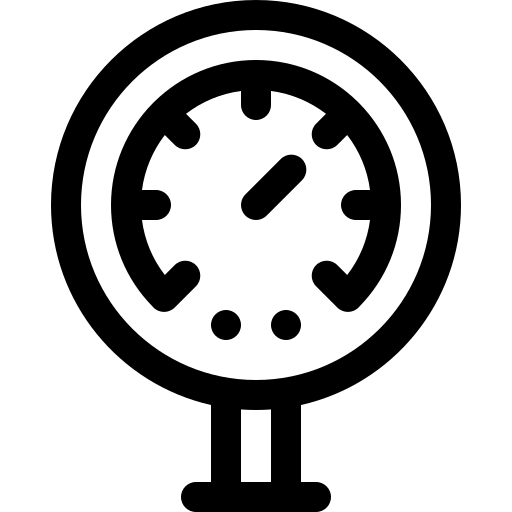
\includegraphics[width=0.5cm]{PressureGuageIcon.png}};
  \node at (1,0.91) {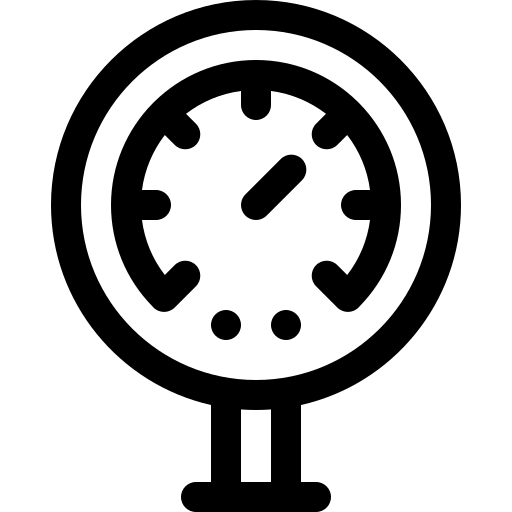
\includegraphics[width=0.5cm]{PressureGuageIcon.png}};

\draw (0,0) .. controls (0.98,1.05) and (1.02,1.05) .. (2,0);
\draw (1.1,1.05) node[anchor=north west] {$Pressure=62psi$};
\draw (-0.65,0.5) node[anchor=north east] {$Flow=120 gpm$};
\draw (-0.65,0.3) node[anchor=north east] {$Pressure=100psi$};
\end{tikzpicture}\\
\vspace{0.2cm}
Total headloss = Headloss due to elevation gain + Headloss due to friction\\
\vspace{0.2cm}
$\implies$ Headloss due to friction = Total headloss - Headloss due to elevation gain\\
\vspace{0.2cm}
Total headloss = $(100 - 62)\enspace \cancel{psi}* \dfrac{ft \enspace head}{0.433\cancel{psi}}=87.8 ft $\\
Headloss due to elevation gain = $60 \enspace ft $\\
$\implies$ Headloss due to friction = $87.8-60=\boxed{27.8 \enspace ft}$\\
\vspace{0.2cm}
 \item Find the force on a 12-inch valve if the water pressure within the line is 60 psi. Express your answer in tons.

$\textrm{Force}= \textrm{Pressure} \times \textrm{Area}$\\
\vspace{0.3cm}
$\implies 60 \enspace \dfrac{\mathrm{lbs}}{\mathrm{in^2}}*0.785 *(12 \mathrm{in})^2*\dfrac{1 \mathrm{ton}}{2000 \mathrm{lbs}} =\boxed{3.39 \enspace\mathrm{tons}}$
\vspace{0.3cm}

\item A water tank is 15 feet deep and 30 feet in diameter. What is the force exerted on a 6-inch valve at the bottom of the tank?\\
\vspace{0.5cm}
$\textrm{Force}= \textrm{Pressure} \times \textrm{Area}$\\
\vspace{0.5cm}
$\implies 15 \enspace\mathrm{ft}* \dfrac{0.433 \enspace \mathrm{psi}}{\mathrm{ft}}*0.785 *(6 \mathrm{in})^2 =\boxed{183 \enspace\mathrm{lbs}}$\\


\item The efficiency of a well pump is determined to be $75 \%$. The efficiency of the motor is estimated at $94 \%$. What is the efficiency of the well?\\
 \vspace{0.2cm}
Solution:\\ 
 \vspace{0.2cm}
$Well \enspace efficiency=\eta_m * \eta_p \implies 0.94 \times 0.75=0.705 \times 100=\boxed{71 \%}$
 \vspace{0.2cm}

  \item Water is being pumped from a reservoir to a storage tank on a hill. The elevation difference between water levels is 1200 feet. Find the pump size (in Hp) required to fill the tank at a rate of 120 gpm.\\
  \vspace{0.2cm}
\begin{tikzpicture}[scale=1]
\draw (0,0) .. controls (1.98,3.5) and (2.02,3.5) .. (4,0);
\node[cylinder, 
    draw = violet, 
    text = purple,
    cylinder uses custom fill, 
    cylinder body fill = blue!10, 
    cylinder end fill = magenta!40,
    aspect = 0.1, 
    shape border rotate = 90] (c) at (2,3.0) {Storage};
\node[cylinder, 
    draw = violet, 
    text = purple,
    cylinder uses custom fill, 
    %cylinder body fill = magenta!10, 
    %cylinder end fill = magenta!40,
    minimum size = 0.3cm, aspect = 0.1,
    shape border rotate = 90] (c) at (2,3.5) {\hspace{0.25cm}{Water}\hspace{0.25cm}};

  \node at (-3,0.1) {\includegraphics[width=3cm]{PumpIcon.png}};
   \node at (-3,-0.8) {
\includegraphics[width=2cm]{WaterReservoirIcon.png}};
   
\draw [ultra thick, -] (-3,-.9) -- (-3,0) node [midway, below] {};
\draw [ultra thick, -] (-3.28,0.63) -- (-3.28,3.1) node [midway, below] {};
\draw [ultra thick, ->] (-3.28,3.1) -- (1.2,3.1) node [midway, below] {};
\draw [ultra thick, ->] (-3.28,3.1) -- (1.2,3.1) node [midway, below] {};
\draw[dashed] (-1.8,-1) -- (2.5,-1);
\draw [<->] (2,-1) -- (2,3.25) node [midway, below] {\hspace{5cm}Elevation difference = 1200 ft};
\draw (0.5,3.7) node[anchor=north east] {$Flow = 120 gpm$};
\end{tikzpicture}\\
\vspace{0.2cm}
Solution:\\
\vspace{0.2cm}
water Hp = flow * head\\
$120GPM*1,200ft*\dfrac{Hp}{3,960 GPM-ft}=\boxed{Water \enspace Hp = 36.4Hp}$\\
\item If a pump is operating at 2,200 gpm and 60 feet of head, what is the water horsepower? If the pump efficiency is 71\%, what is the brake horsepower?\\
\vspace{0.2cm}
Solution:\\
\vspace{0.2cm}
water Hp = flow * head\\
$2,200GPM*60ft*\dfrac{Hp}{3,960 GPM-ft}=\boxed{Water \enspace Hp = 33.3Hp}$\\
\vspace{0.4cm}
pump Hp = brake Hp * pump efficiency\\
$brake \enspace Hp = \dfrac{33.3}{0.71}=\boxed{Brake \enspace Hp=47Hp}$
 \vspace{0.2cm}


\item The water horsepower of a pump is $10 \mathrm{Hp}$ and the brake horsepower output of the motor is $15.4 \mathrm{Hp}$. What is the efficiency of the pump?\\
\vspace{0.2cm}
Solution:\\ 
 \vspace{0.2cm}
 \vspace{0.4cm}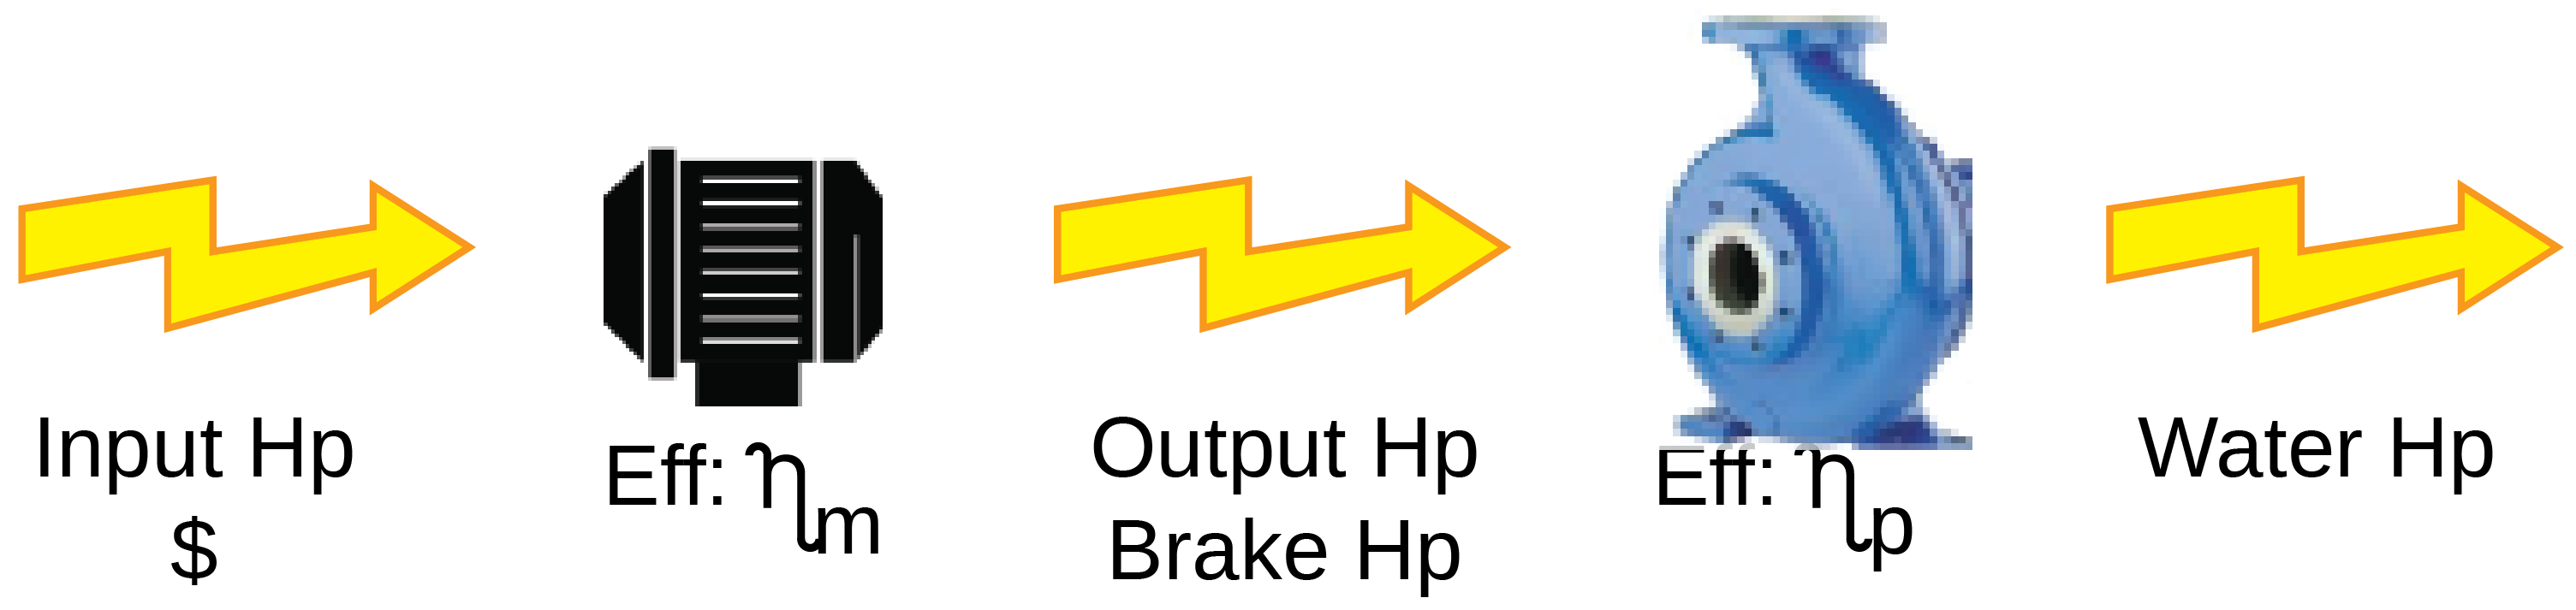
\includegraphics[scale=0.08]{PumpProblem}\\
 \vspace{0.2cm}
 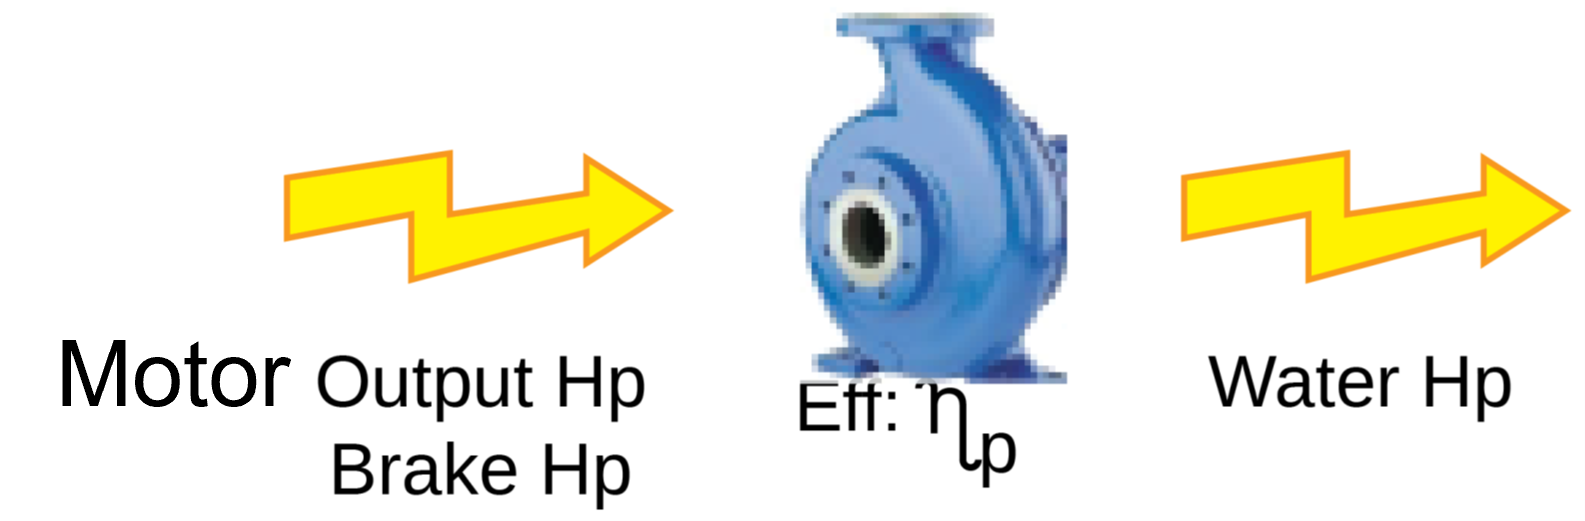
\includegraphics[scale=0.32]{PumpingProblemPump}
 $\eta_p=\dfrac{10 \mathrm{BHp}}{15.4 \mathrm{EHp}} \times 100=\boxed{65 \%}$\\
 \vspace{0.2cm}
 \item The water horsepower of a pump is $25 \mathrm{Hp}$ and the brake horsepower output of the motor is $48 \mathrm{Hp}$. What is the efficiency of the pump?\\
 Solution:\\
  \vspace{0.2cm}
 \vspace{0.32cm}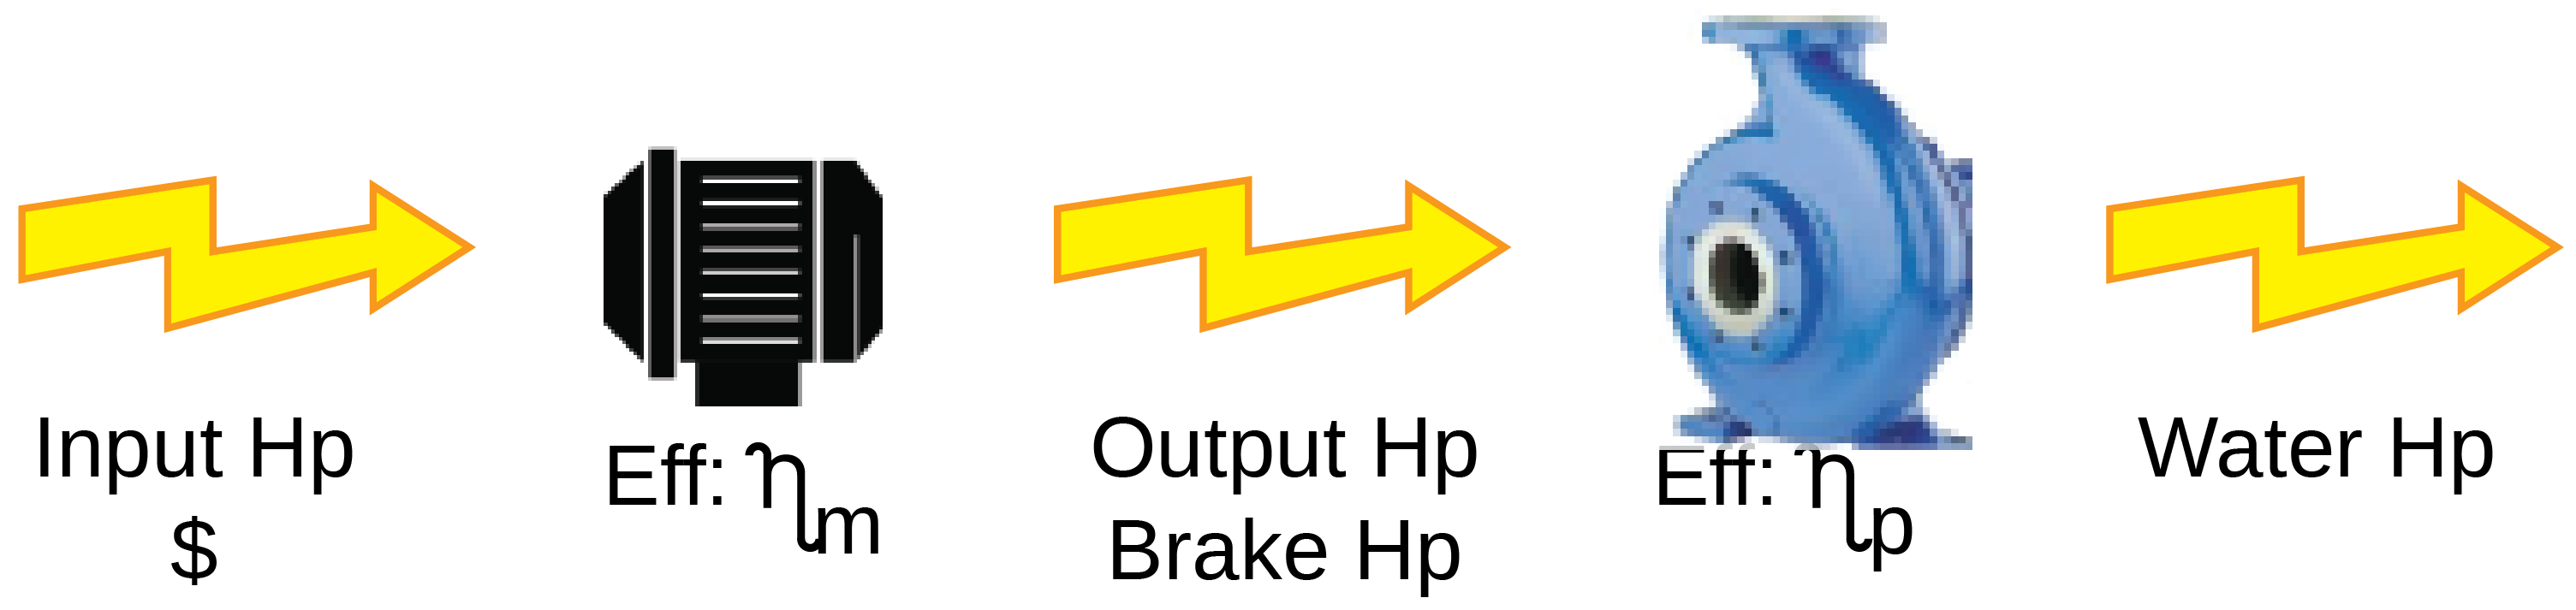
\includegraphics[scale=0.08]{PumpProblem}\\
 \vspace{0.2cm}
 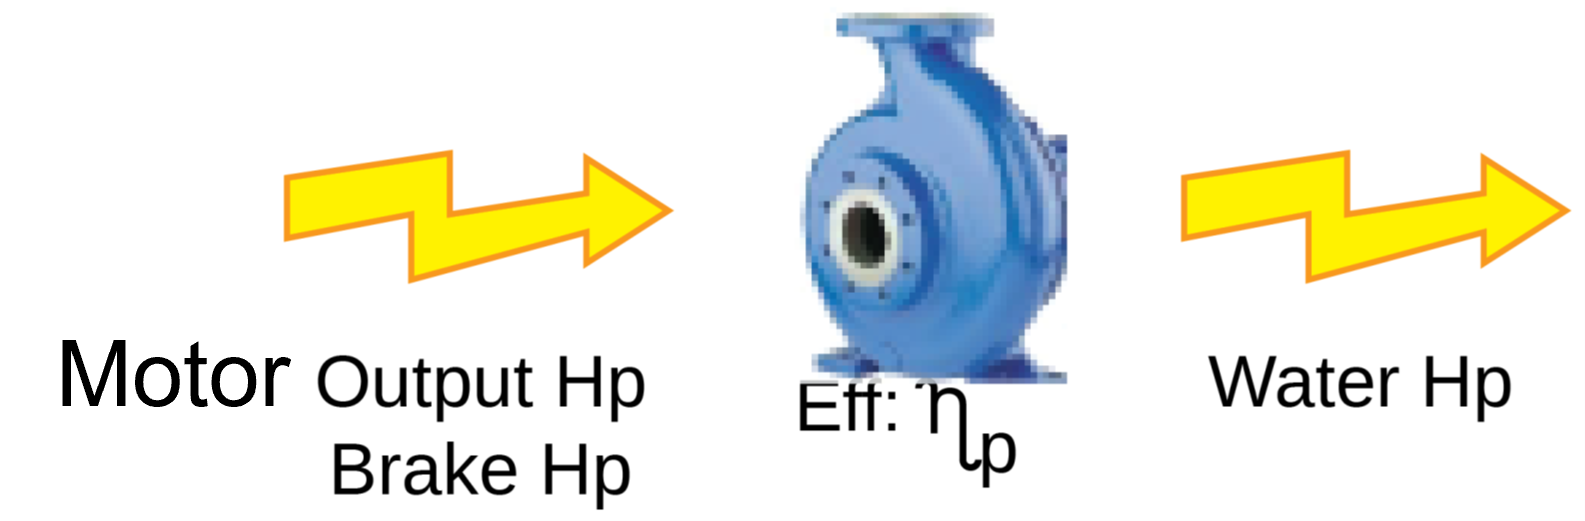
\includegraphics[scale=0.4]{PumpingProblemPump}
 \vspace{0.2cm}
$\eta_p=\dfrac{25 \mathrm{\enspace Water \enspace Hp}}{48 \mathrm{\enspace brake \enspace Hp}} \times 100=\boxed{52 \%}$
  \vspace{0.4cm}
\end{enumerate}
\newpage
\section{Week 6 Assessment}
% \textbf{Multiple Choice}
\begin{enumerate}[1.]
\item What federal law is designed to protect the safety and health of operators?\\
*a. OSHA\\
b. FMLA\\
c. FLSA\\
d. ADEA\\
\item What are the two most important safety concerns when entering a confined space?\\
a. Corrosive chemicals and falls\\
b. Bad odors and claustrophobia\\
c. Extreme air temperatures and slippery surfaces\\
*d. Oxygen deficiency and hazardous gases\\
\item Which document provides a profile of hazardous substances?\\
a. CERCLA\\
b. SARA\\
c. CFR\\
*d. SDS\\
\item What is the purpose of a pump guard?\\
a. Allows operators to turn off pump in emergency situations\\
b. Notifies operators of excessive temperatures\\
c. Allows operators to pump against a closed discharge valve\\
*d. Protects operators from rotating parts\\
\item Atmosphere is considered oxygen deficient when the oxygen level is below\\
a. $21.5 \%$\\
b. $20 \%$\\
*c. $19.5 \%$\\
d. $17 \%$\\
\item Employee hazards include\\
a. Noxious or toxic gases or vapors\\
b. Oxygen deficiency\\
c. Physical injuries\\
*d. All of the above\\
\item Before entering a permit-required confined space, you must:\\
a. Check the atmosphere with a calibrated gas detector.\\
b. Make notification that personnel are entering the space.\\
c. Lock out and tag out all equipment.\\
*d. All of the above.\\
\item When making a sulfuric acid dilution, the appropriate method is:\\
a. Add the water to the acid.\\
*b. Add the acid to the water.\\
c. Add both at the same time.\\
d. None of the above.\\
\item When manually lifting any object, be sure to\\
a. Hold it at arm's length.\\
b. Keep your back bent and hold it low.\\
*c. Keep it close to your body and use leg strength.\\
d. Keep your knees locked and bend at the waist.\\
\item What is the proper slope of a ladder?\\
*a. Every 4 feet up the ladder is 1 foot out from the wall.\\
b. Every 5 feet up the ladder is 1 foot out from the wall.\\
c. Every 6 feet up the ladder is 1 foot out from the wall.\\
d. Every 7 feet up the ladder is 1 foot out from the wall.\\
\item When working on a chemical feed pump, what of the following is not required?\\
a. Nitrile gloves.\\
b. Safety glasses.\\
*c. Leather work gloves.\\
d. Full face shield.\\
\item When must the atmosphere of a confined space be tested?\\
a. Only before a worker enters\\
b. Never, if adequate ventilation exists\\
*c. Continuously\\
d. Only if welding or painting is being performed\\
\item Some gases in a confined space can be:\\
a. Colorless\\
b. Odorless\\
c. Deadly\\
*d. All of the above\\
\item Why should you contact other area companies with underground utilities before starting an underground repair job?\\
a. To determine if there have been recent excavations in that location\\
*b. To ask these companies to mark the location of their utilities in the area of the repair job\\
c. To see if they also have excavating to do in the area\\
d. To see if they will help route traffic while you are doing the repair job\\
\item The only acceptable breathing device to wear while handling chlorine leaks is the\\
a. Activated carbon canister type\\
b. Potassium tetroxide canister type\\
*c. Self-contained breathing apparatus\\
d. Oxygen supply apparatus\\
  \end{enumerate}
